\todo[inline]{Explain the used metrics and how they relate to hypothesis}
\todo[inline]{Introduce the baselines, explain how they relate to the hypothesis, why they - are chosen, how they differ}
\todo[inline]{Explain methodology, why the chosen metric really captures the problem at - hand}
\todo[inline]{Work out differences of graph types, find similarities across datasets}
\todo[inline]{Provide the questions that are relevant for the hypothesis}
\todo[inline]{Answer these questions through metrics/results}

In order to test the hypothesis, we first derive a number of questions from the hypothesis.
We will also often compare the results on these questions for concept maps to co-occurrence graphs to find differences. While the comparison to co-occurrence graphs is interesting by itself, it is not entirely fair since co-occurrence graphs have far more nodes than concept maps.
Nevertheless, co-occurrence graphs capture the words of a text completely.

In the next chapter, we will give the results to the questions we posed in this chapter and also discuss their significance to the hypothesis.

\labelsubsection{Experiments}{subsec:experiments}
\todo[inline]{Test the hypothesis}
\todo[inline]{Tables with results}
\todo[inline]{Mention difficulties and possible solutions}
\todo[inline]{Add runtime analysis}

\subquestion{How diverse is the structure of the concept maps?}{question:structure_diversity}
When the structure of the graphs is mostly homogeneous or the structural differences are not distinct between graphs of different classes, the structure by itself will most likely not contribute to the classification performance.
When comparing the graph similarity under some graph kernel, the graphs of a given class should be distinguishable from the graphs of the other classes.

To explore the variance in the structure of concept maps, we look at the following metrics:
\begin{enumerate}
    \item{Histogram of the number of connected components}
    \item{Histogram of the size of connected components}
    \item{Average node/edge ratio}
\end{enumerate}

All these methods aim to find out the diversity of the connectedness of concept maps. There a lot of other metrics, but as we will see later on these metrics suffice to get a good picture about the structure of the concept maps.

\subquestion{How important is the structure of concept maps compared to the content?}{question:importance_structure}
Another important question is the relative importance of the structure compared to the content, or the labels. For this, we use the following methodology:

\begin{quote}
Compare results from structure-only graph kernels with the results of graph kernels that use a) only content and b) both content and structure.
\end{quote}

For the content-only kernel, we will simply count the number of occurrences of labels in the graphs and essentially create a bag-of-words representation of the graph. The kernel then creates the similarity score by calculating the inner product on these vector representations, effectively counting the number of common labels.

For the structure-only kernel, we will use a modified version of the Weisfeiler-Lehman kernel: before executing the WL kernel on the graphs, we first discard all labels on the graph. All nodes of all graphs get the same label. This way, only the structure gets used for the similarity score.

For the structure-and-content kernel, we use the plain Weisfeiler-Lehman graph kernel.

\subquestion{How does the classification results of co-occurrence graphs compare to concept maps?}{question:comparison_coo}
We compare the classification results for concept maps and co-occurrence graphs. As noted before, this comparison is slightly unfair since co-occurrence graphs have far more content than concept maps.
Nevertheless, it is an interesting baseline for graph-based text-classification.

\subquestion{How does the classification performance compare to non-structural, text-based approaches?}{question:comparison_text}

\subquestion{How useful are the concept maps combined with text classification?}{question:comparison_combined}
When concept maps indeed have a structure that is useful for classification and which is not captured by text-only approaches, the classification performance should increase when combining graph- and text based approaches.

\subsubsection{Baselines}
\paragraph{Preprocessing}
Before creating the vector representations of the text documents or the creation of the co-occurrence graphs and concept maps, we first pre-processed the plain text by

\begin{itemize}
\item{lowercasing the text,}
\item{removing non-printable characters,}
\item{replacing numbers with a \textit{NUMBER} placeholder,}
\item{replacing tabs and newlines with a space,}
\item{and normalizing the whitespace (eg. replacing multiple spaces with a single space)}
\end{itemize}
These pre-processing steps are similar to the pre-processing done in \cite{Cachopo2007}.

\todo[inline]{Filtered out only nouns?}

\paragraph{Text-based representations}
For the text classification pipeline, we used two different vectorization algorithms, namely
\begin{itemize}
\item{Bag Of Words (BoW): this vectorizer simply gathers all words in the corpus and creates a mapping between words and indices (ids). Then it creates a vector representation for each text so that the i-th vector component  is the count of the corresponding word in the text. Ie. $i$ is the index of the word in the mapping.}
\item{Term-Frequency-Inverse-Document-Frequency (TfIdf): this approach is similar to BoW. Instead of using only the counts of a word in the text, this approach also incorporates the term frequency and the inverse document frequency of the words to the vector representation (see below).}
\end{itemize}
Both approaches can also be extended by not only utilizing single words (unigrams) but n-grams, too. A word n-gram consists of $n$ words that appear consecutively in the text.
For example, the sentence ``This is a sentence." has the following 2-grams, or bigrams: $\{ (This, is), (is, a), (a, sentence) \}$.
For our purposes, we looked at n-grams of lengths (1, 1), (1, 2) and (2, 2).
Note that word n-grams do not take word inversion into account, ie. the bigram (a, b) is not the same as (b, a).

\todo[inline]{Explain ranges of n-grams}
\todo[inline]{Explain tfidf}

\paragraph{Graph-based representations}
To compare the performance of concept maps with other graphs, we generated co-occurrence graphs with window sizes of $\{1, 2, 3\}$.

\todo[inline]{Co-occurrence and concept maps}
\todo[inline]{Mention filtering by nouns}
\todo[inline]{Window sizes}

\begin{figure}[ht]
\centering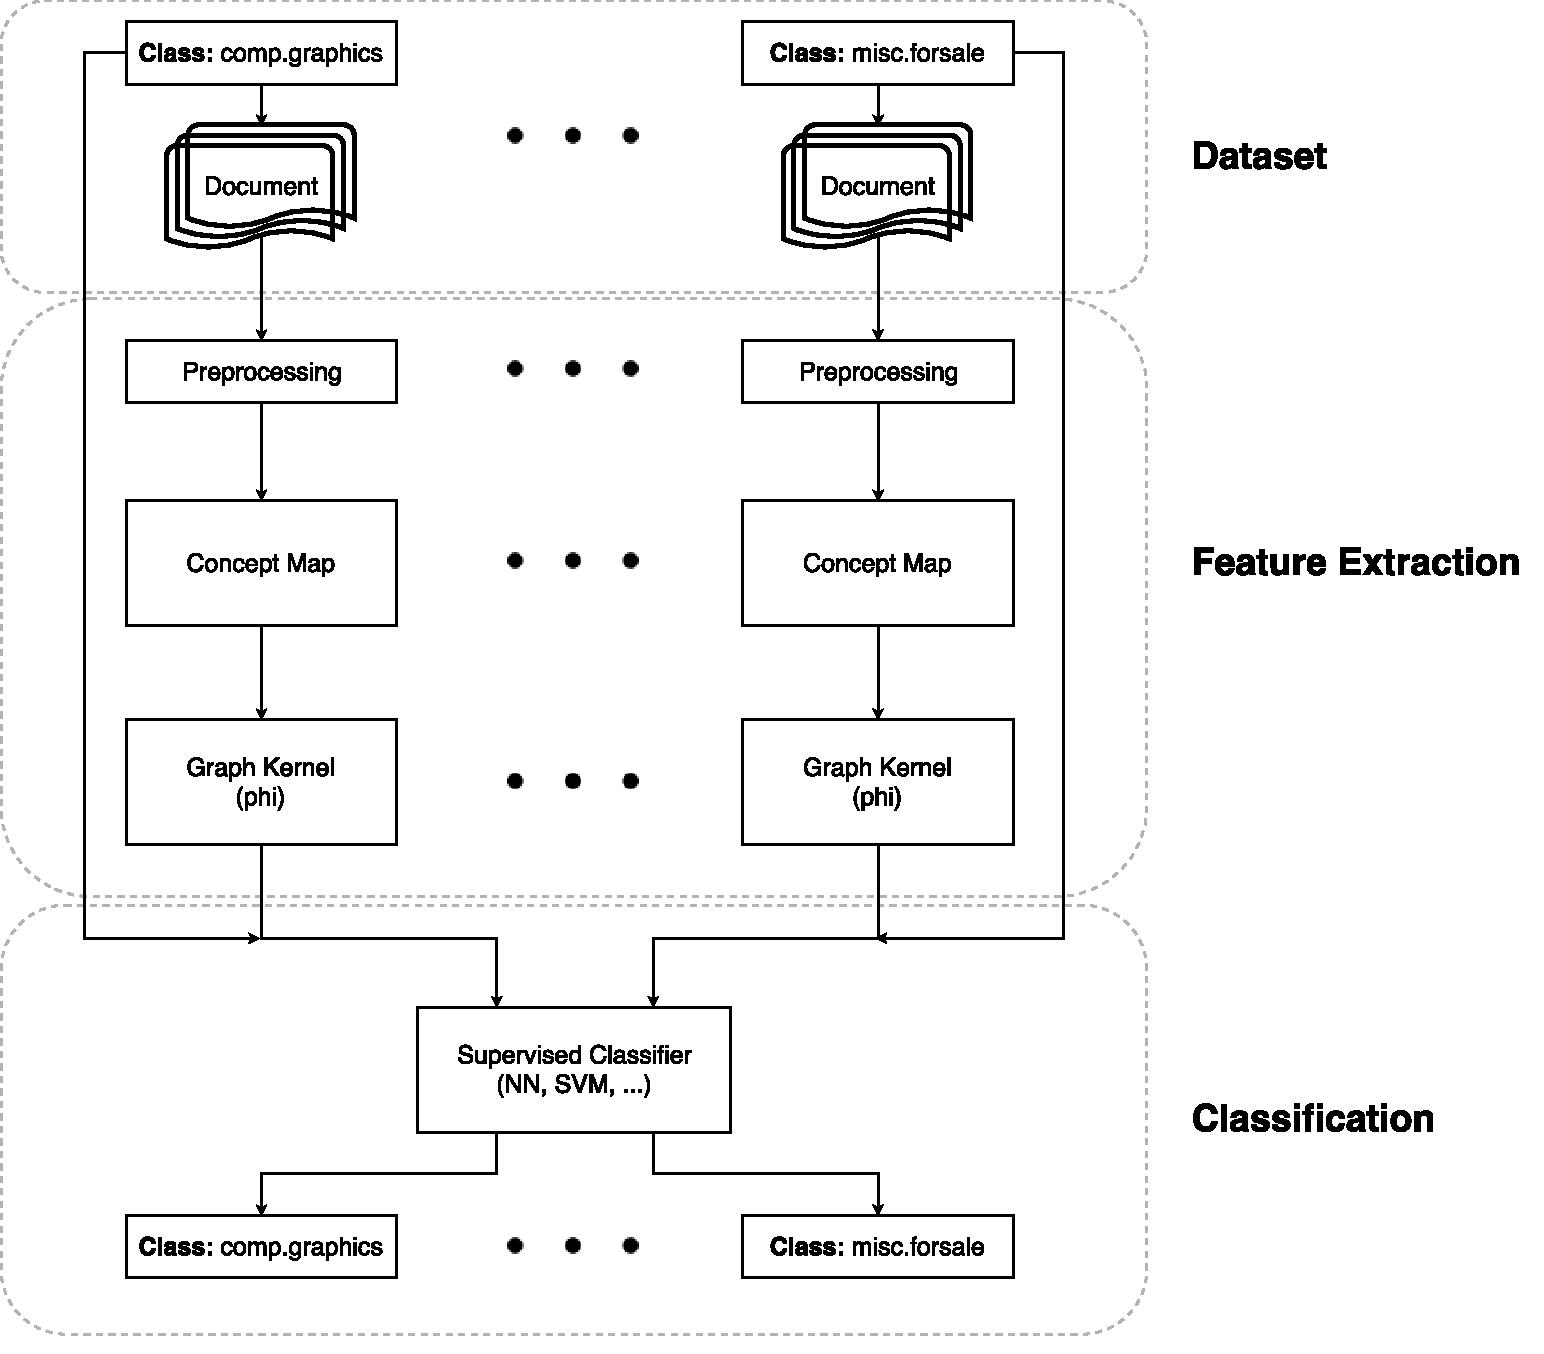
\includegraphics[width=0.6\linewidth]{assets/figures/approach.pdf}
\caption{Graph kernel based classification pipeline.}
\end{figure}
\todo[inline]{Add diagram for gram-matrix based classification.}

\labelsubsection{Datasets}{subsec:datasets}
\todo[inline]{Statistics about datasets and derived graphs}
\todo[inline]{Skewed classes}
\todo[inline]{Give hints where to download the datasets from}
\todo[inline]{A script to download all datasets is also provided alongside the other code}

\paragraph{ling-spam}
The Ling-Spam dataset was created by Ion Androutsopoulos et al. \cite{Androutsopoulos2000}.
The corpus contains the texts, which are categorized as ``spam" and ``no spam". For this work, we used the version which can be downloaded from here\footnote{\url{http://csmining.org/index.php/ling-spam-datasets.html}}.

\paragraph{ng20}
The 20 Newsgroup corpus \cite{Lang} consists of posts from an internet forum. They are labeled with 20 different classes, corresponding to the topic they have been posted on. The texts are mostly informal and consist of discussions between users of the forum.
For this dataset, as an additional pre-processing step, we remove the headers and footers from the documents.

While the classes are nearly evenly distributed, some classes are highly correlated. This adds an additional difficulty to the task.

\todo[inline]{Explain correlation more throughly}

\paragraph{reuters-21578}
\footnote{\url{http://www.nltk.org/book/ch02.html#reuters-corpus}}
\todo[inline]{Documents came from Reuters newswire in 1987.}

\paragraph{r8}
This dataset is a subset of the \textit{reuters-21578} dataset.
It consists of the 8 most frequent classes of the \textit{reuters-21578} dataset, ie. the 8 classes with the most documents.

\paragraph{review\_polarity}
\cite{Pang2004}.
\footnote{\url{http://www.cs.cornell.edu/people/pabo/movie-review-data/review_polarity.tar.gz}}

\paragraph{rotten\_imdb}
\cite{Pang2004}.
\footnote{\url{http://www.cs.cornell.edu/people/pabo/movie-review-data/rotten_imdb.tar.gz}}

\paragraph{tagmynews}
\footnote{\url{http://acube.di.unipi.it/repo/news.gz}}

\paragraph{webkb}
\footnote{\url{http://www.cs.cmu.edu/afs/cs/project/theo-20/www/data/}}

\begin{figure}[ht]
\centering
\begin{tabular}{lrrrr}
{} &  \# docs &  \# classes &  median \#words/doc &  \#uniq. words/\#words \\
\midrule
ling-spam       & 18846 & 20 & 277 & 0.20 \\
ng20            & 2893 & 2 & 79 & 0.22 \\
reuters-21578   & 18846 & 20 & 94 & 0.07 \\
review\_polarity & 13328 & 90 & 589 & 0.16 \\
rotten\_imdb     & 2000 & 2 & 19 & 0.34 \\
tagmynews       & 10000 & 2 & 24 & 0.11 \\
webkb           & 32600 & 7 & 158 & 0.15 \\
\bottomrule
\end{tabular}
\caption{Dataset statistics}
\end{figure}


\labelsubsection{Methods}{subsec:methods}

\subsubsection{Cross-Validation}
For all the classification tasks we used train-/validation- and test sets.
The split is done as follows: 85\% for train- and validation set together and 15\% for the validation set.
We then use stratified k-fold cross-validation to further split the train- and validation set. In our case, we used $k = 3$, meaning that $\frac{2}{3}$ of the dataset is used for training, and the rest for validation.
The stratification ensures that the class distribution in the train set is (nearly) the same as in the validation set.

\subsubsection{Metrics}
We evaluated a number of metrics for each classification task, namely: 
recall, precision, accuracy and the F1-score. We mostly focus on the F1-score since it captures the overall performance of classification algorithms.

\subsubsection{Significance tests}
When comparing two models we used the permutation test, or exact test, to test the significance of the difference in performance of these two approaches.
The permutation test tests whether the observed difference of the performances of the two approaches is the product of chance.
The test only returns a probability for observing a given performance difference. The test does not give a definite answer whether the difference was due to chance.
When the probability of observing the difference by chance is below a given threshold, we say that the test shows that the approaches really differ in their performance.
For our case, we chose the threshold of 0.5\%.

\begin{figure}[ht]
\centering
\missingfigure[figcolor=white]{}
\caption{Permutation test}
\end{figure}

\todo[inline]{\url{https://stats.stackexchange.com/questions/104040/resampling-simulation-methods-monte-carlo-bootstrapping-jackknifing-cross}}

\labelsubsection{Implementation}{sec:implementation}
For the implementation of all these experiments, we used mostly Python.
\todo[inline]{Scikit-learn, networkx, \dots}
\todo[inline]{Code by Tobias to extract concept maps}
